\documentclass{beamer}
\usepackage{amsmath}
\usepackage[english]{babel} %set language; note: after changing this, you need to delete all auxiliary files to recompile
\usepackage[utf8]{inputenc} %define file encoding; latin1 is the other often used option
\usepackage{csquotes} % provides context sensitive quotation facilities
\usepackage{graphicx} %allows for inserting figures
\usepackage{booktabs} % for table formatting without vertical lines
\usepackage{textcomp} % allow for example using the Euro sign with \texteuro
\usepackage{stackengine}
\usepackage{wasysym}
\usepackage{tikzsymbols}
\usepackage{textcomp}
% ELIMINAR COMANDOS DE NAVEGACION%%%%%%%%%%%
\setbeamertemplate{navigation symbols}

%\newcommand{\bubblethis}[2]{
 %       \tikz[remember picture,baseline]{\node[anchor=base,inner sep=0,outer sep=0]%
 %       (#1) {\underline{#1}};\node[overlay,cloud callout,callout relative pointer={(0.2cm,-0.7cm)},%
 %       aspect=2.5,fill=yellow!90] at ($(#1.north)+(-0.5cm,1.6cm)$) {#2};}%
 %   }%
%\tikzset{face/.style={shape=circle,minimum size=4ex,shading=radial,outer sep=0pt,
 %       inner color=white!50!yellow,outer color= yellow!70!orange}}

%% Some commands to make the code easier
\newcommand{\emoticon}[1][]{%
  \node[face,#1] (emoticon) {};
  %% The eyes are fixed.
  \draw[fill=white] (-1ex,0ex) ..controls (-0.5ex,0.2ex)and(0.5ex,0.2ex)..
        (1ex,0.0ex) ..controls ( 1.5ex,1.5ex)and( 0.2ex,1.7ex)..
        (0ex,0.4ex) ..controls (-0.2ex,1.7ex)and(-1.5ex,1.5ex)..
        (-1ex,0ex)--cycle;}
\newcommand{\pupils}{
  %% standard pupils
  \fill[shift={(0.5ex,0.5ex)},rotate=80] 
       (0,0) ellipse (0.3ex and 0.15ex);
  \fill[shift={(-0.5ex,0.5ex)},rotate=100] 
       (0,0) ellipse (0.3ex and 0.15ex);}

\newcommand{\emoticonname}[1]{
  \node[below=1ex of emoticon,font=\footnotesize,
        minimum width=4cm]{#1};}
\usepackage{scalerel}
\usetikzlibrary{positioning}
\usepackage{xcolor,amssymb}
\newcommand\dangersignb[1][2ex]{%
  \scaleto{\stackengine{0.3pt}{\scalebox{1.1}[.9]{%
  \color{red}$\blacktriangle$}}{\tiny\bfseries !}{O}{c}{F}{F}{L}}{#1}%
}
\newcommand\dangersignw[1][2ex]{%
  \scaleto{\stackengine{0.3pt}{\scalebox{1.1}[.9]{%
  \color{red}$\blacktriangle$}}{\color{white}\tiny\bfseries !}{O}{c}{F}{F}{L}}{#1}%
}
\usepackage{fontawesome} % Social Icons
\usepackage{epstopdf} % allow embedding eps-figures
\usepackage{tikz} % allows drawing figures
\usepackage{amsmath,amssymb,amsthm} %advanced math facilities
\usepackage{lmodern} %uses font that support italic and bold at the same time
\usepackage{hyperref}
\usepackage{tikz}
\usepackage{tcolorbox}

\usefonttheme[onlymath]{serif} %set math font to serif ones

\definecolor{beamerblue}{rgb}{0.2,0.2,0.7} %define beamerblue color for later use

%%% defines highlight command to set text blue
\newcommand{\highlight}[1]{{\color{blue}{#1}}}


%%%%%%% commands defining backup slides so that frame numbering is correct

\newcommand{\backupbegin}{
   \newcounter{framenumberappendix}
   \setcounter{framenumberappendix}{\value{framenumber}}
}
\newcommand{\backupend}{
   \addtocounter{framenumberappendix}{-\value{framenumber}}
   \addtocounter{framenumber}{\value{framenumberappendix}}
}

%%%% end of defining backup slides

%Specify figure caption, see also http://tex.stackexchange.com/questions/155738/caption-package-not-working-with-beamer
\setbeamertemplate{caption}{\insertcaption} %redefines caption to remove label "Figure".
%\setbeamerfont{caption}{size=\scriptsize,shape=\itshape,series=\bfseries} %sets figure  caption bold and italic and makes it smaller

\newtcolorbox{boxA}{
    fontupper = \bf,
    boxrule = 1.5pt,
    colframe = black % frame color
}

\usetheme{Boadilla}
% --------------------
% Overall information
% --------------------
\title[Economía I]{Economía I \vspace{4mm}
\\ Magistral 13: Competencia Imperfecta}
\date{}
\author[Riottini]{Riottini Franco}
\vspace{0.4cm}
\institute[]{Universidad de San Andrés} 

\begin{document}

\begin{frame}
    \titlepage
    \centering
    
\includegraphics[scale=0.2]{../Figures/logoUDESA.jpg} 
\end{frame}


\begin{frame}{El problema de la firma}
    \begin{itemize}
        \item Una vez que conocemos la demanda... ¿cómo se elige cuánto producir y el precio que cobrar?
        \item El problema principal de \textbf{toda} empresa es el de la maximización del beneficios
        \begin{itemize}
            \item ¿Qué es el beneficio? Beneficio = Ingresos totales – Costos totales
            \item ¿Qué es el ingreso total? El valor de la producción al precio ofrecido (p·q)
            \item ¿Qué es el costo total? Los costos por unidad, por la cantidad de unidades producidas (c·q)
        \end{itemize}
    \end{itemize}
\end{frame}

\begin{frame}{Monopolios}
    \begin{itemize}
        \item Hay una unica empresa que vende productos especializados tienen un alto poder de mercado.
        \begin{itemize}
            \item Enfrentan poca competencia, tienen una demanda inelástica, y pueden fijar precio superior al costo marginal sin perder todos sus clientes.
            \item Las barreras de entrada ayudan a generar rentas.
            \begin{itemize}
                \item Beneficios económicos por encima de los costos de producción.
                \item Por eso las barreras a la entrada ¡son el peor enemigo de los economistas (y de la sociedad)!
            \end{itemize}
        \end{itemize}
        \item En estos casos, en equilibrio encontramos una pérdida de peso muerto.
        \begin{itemize}
            \item Tenemos entonces una falla de mercado.
            \item Es decir, los mercados asignan recursos, sin competencia, en una forma no óptima.
        \end{itemize}
    \end{itemize}
\end{frame}


\begin{frame}{Mirando el ingreso total}
    \begin{itemize}
        \item El concepto clave para la decisión del monopolista es el de ingreso marginal
        \begin{itemize}
            \item Que es la variación en los ingresos totales al vender una unidad adicional.
            \item Es el efecto neto de la disminución de los precios y el aumento de la cantidad vendida.
        \end{itemize}
        \item La curva de demanda, veremos, nos determina ingresos marginales decrecientes
        
        \item ¿Cómo cambia el ingreso al aumentar la producción?
        \begin{itemize}
            \item Ahora se vende una unidad más...
            \item ...¡pero todas las vendo a un precio menor!
        \end{itemize}
    \end{itemize}
\end{frame}

\begin{frame}{¿Cómo cambia el ingreso total?}
    \centering
    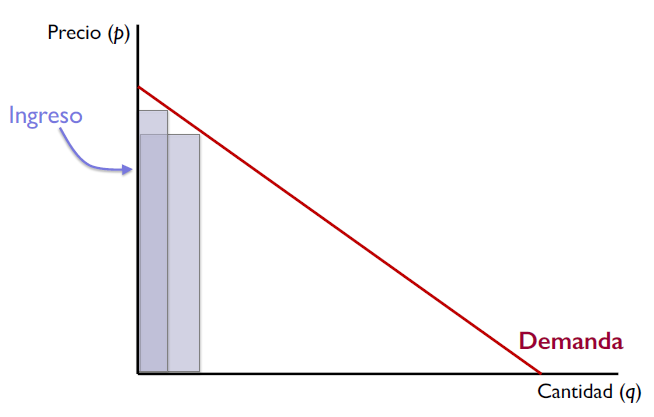
\includegraphics[scale=0.6]{../Figures/Tema_06.30_ingresototal.png}
\end{frame}

\begin{frame}
\frametitle{¿Cómo cambia el ingreso total?}
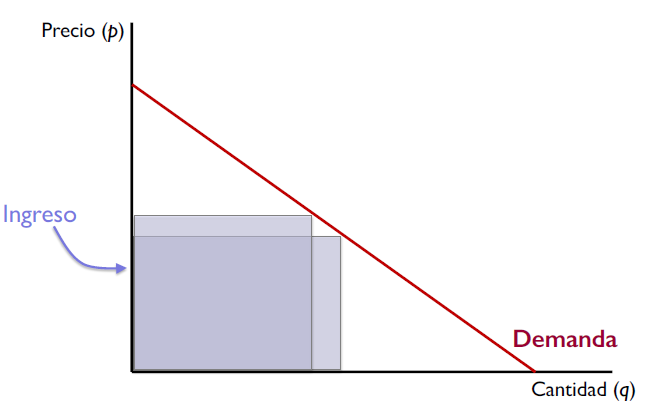
\includegraphics[scale=0.6]{../Figures/Tema_06.31_ingresototal2.png}
\end{frame}

\begin{frame}
\frametitle{¿Cómo cambia el ingreso total?}
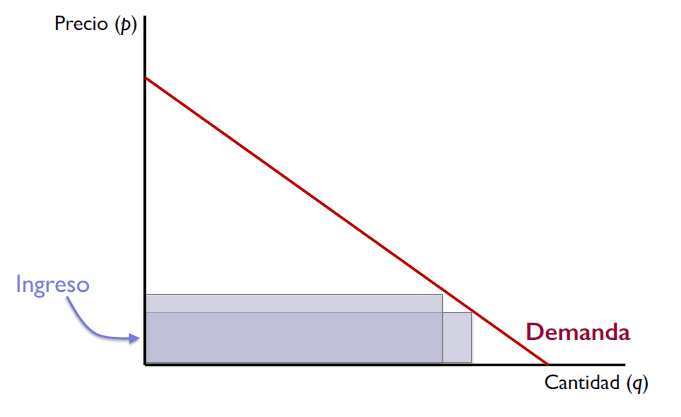
\includegraphics[scale=0.6]{../Figures/Tema_06.32_ingresototal3.png}
\end{frame}

\begin{frame}{El ingreso marginal}
    \centering
    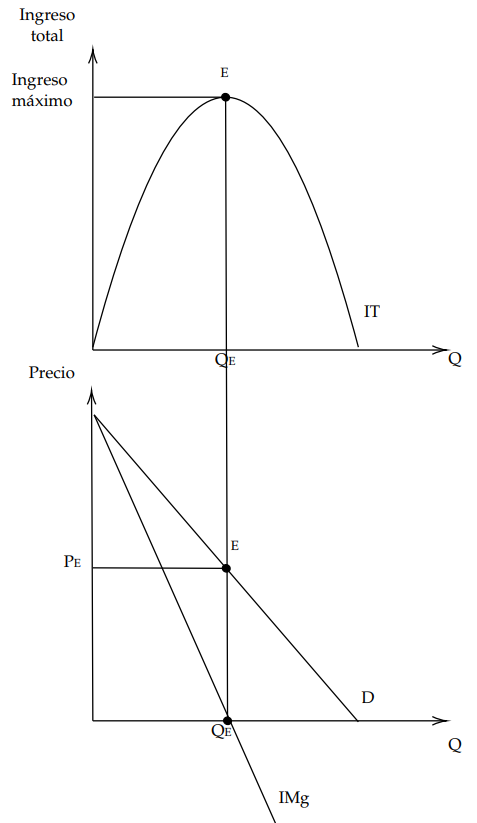
\includegraphics[scale=0.45]{../Figures/C22.4.png}
\end{frame}

\begin{frame}
\frametitle{El ingreso marginal}
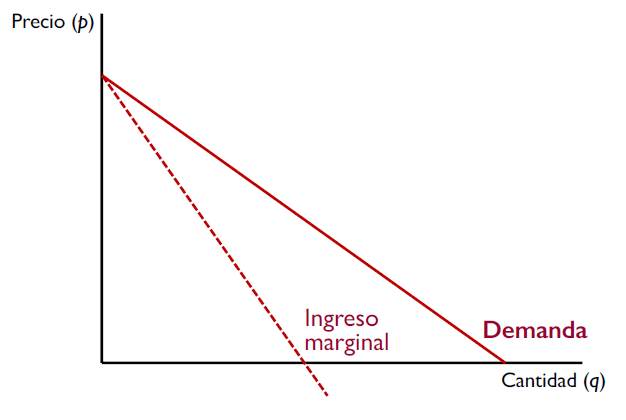
\includegraphics[scale=0.6]{../Figures/Tema_06.33_ingresomarginal.png}
\end{frame}

\begin{frame}
\frametitle{Costo e ingreso marginal}
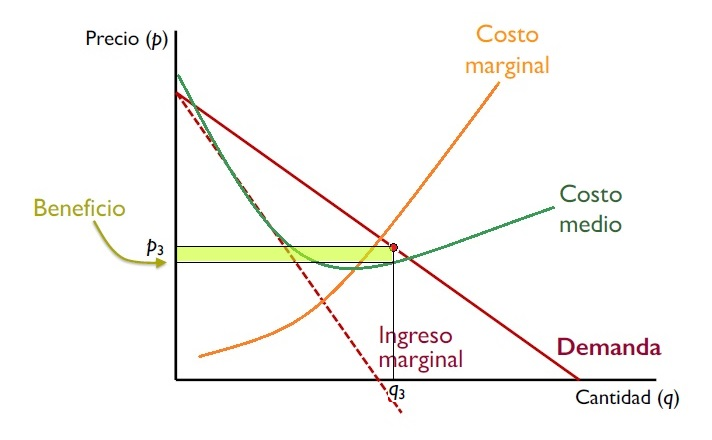
\includegraphics[scale=0.6]{../Figures/Tema_06.36_beneficios3.jpg}
\end{frame}

\begin{frame}
\frametitle{¿Cómo cambian los beneficios?}
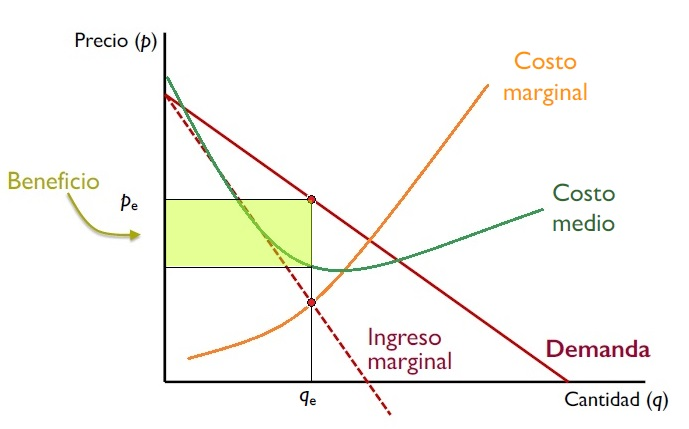
\includegraphics[scale=0.6]{../Figures/Tema_06.35_beneficios2.jpg}
\end{frame}

\begin{frame}
\frametitle{¿Cómo cambian los beneficios?}
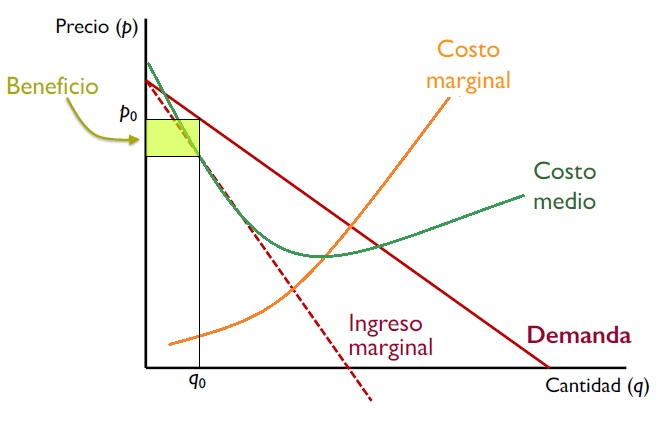
\includegraphics[scale=0.6]{../Figures/Tema_06.34_beneficios.jpg}
\end{frame}

\begin{frame}{La lógica marginal}
    \begin{itemize}
        \item El punto que maximiza el beneficio es donde la curva de IMg cruza la curva de CMg.
        \item Recordemos que

        \[ B = p \cdot q – C(q) = IT(q) - C(q)\]
        \begin{itemize}
            \item Para cualquier valor de $q$, el cambio del beneficio si $q$ fuera aumentado en una unidad sería la diferencia entre el cambio en ingresos, y el cambio en costos:
            
            \begin{center} 
                Beneficio marginal = IMg - CMg 
            \end{center}

            \item Entonces:
            \begin{itemize}
                \item Si $IMg > CMg$ aumentando $q$ se podrían incrementar los beneficios.
                \item Si $IMg < CMg$ el beneficio marginal es negativo, con lo que sería mejor disminuir $q$ para aumentar los beneficios.
            \end{itemize}
        \end{itemize}
    \end{itemize}
\end{frame}

\begin{frame}{Equilibrio del monopolista}
    \centering
    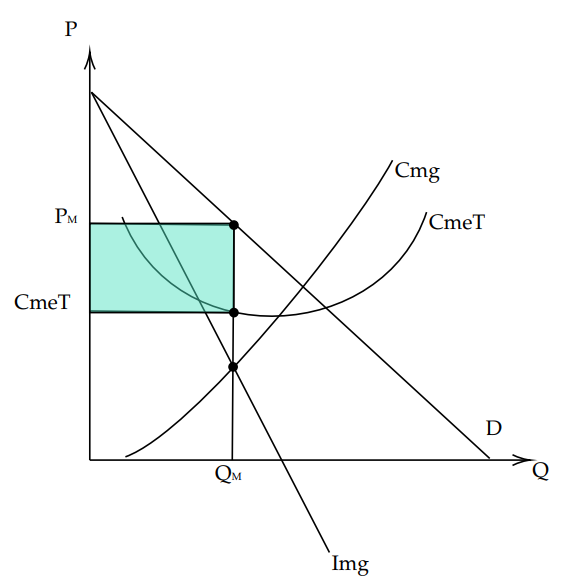
\includegraphics[scale=0.6]{../Figures/C22.5.png}
\end{frame}

\begin{frame}
\frametitle{Excedentes y peso muerto}
\begin{itemize}
    \item Las ganancias totales del intercambio están determinadas por los excedentes de consumidores y productores
    \begin{itemize}
        \item El excedente del consumidor: Diferencia entre disposición a pagar y precio de compra
        \item Excedente del productor: Diferencia entre precio y costo de una unidad adicional
    \end{itemize}
    \item Si no terminamos en una asignación Pareto eficiente tenemos una ‘pérdida de peso muerto’
    \begin{itemize}
        \item Pérdida de excedente total con respecto a una asignación eficiente de Pareto. Es decir, hay ganancias no explotadas del comercio
    \end{itemize}
    \end{itemize}
\end{frame}

%\begin{frame}
%\frametitle{Precios y excedentes}
%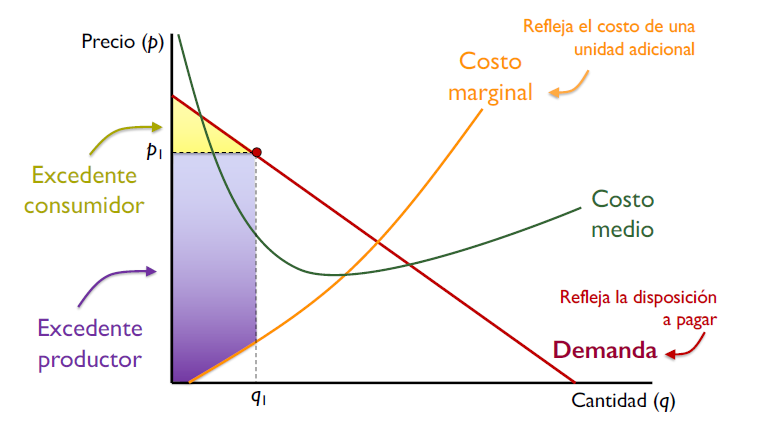
\includegraphics[scale=0.6]{../Figures/Tema_06.38_excedente1.png}
%\end{frame}

%\begin{frame}
%\frametitle{Mejora de Pareto}
%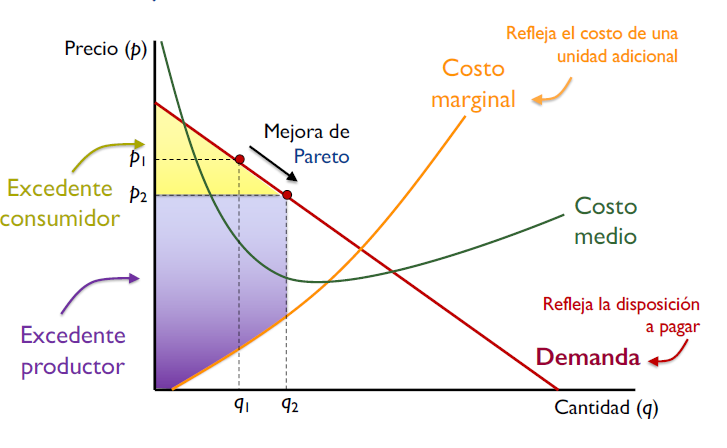
\includegraphics[scale=0.6]{../Figures/Tema_06.39_excedente2.png}
%\end{frame}

\begin{frame}
\frametitle{Eficiencia de Pareto}
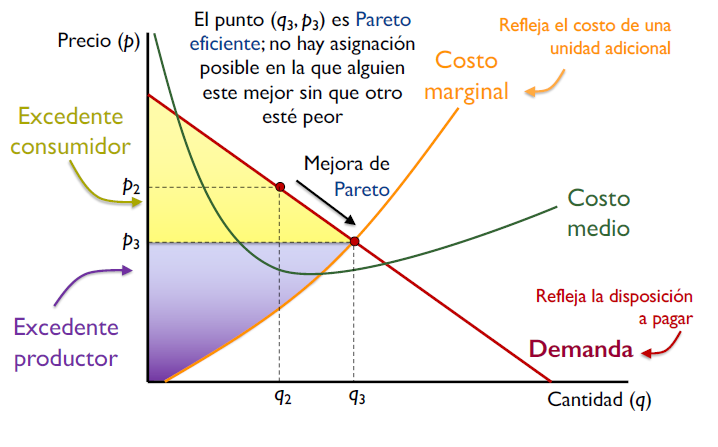
\includegraphics[scale=0.6]{../Figures/Tema_06.40_excedente3.png}
\end{frame}

\begin{frame}
\frametitle{Cuando maximiza la firma}
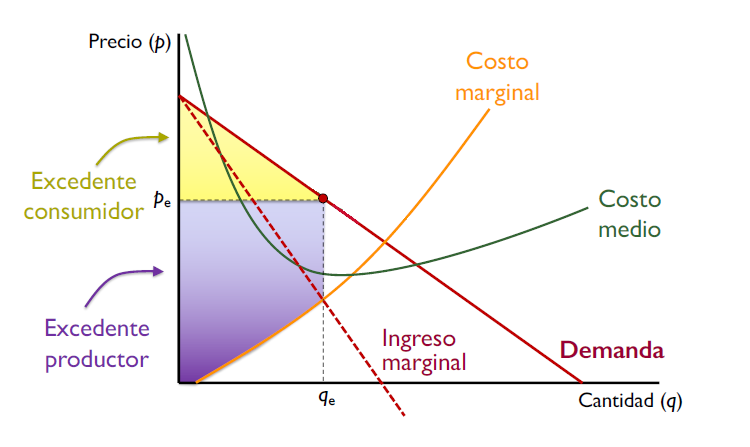
\includegraphics[scale=0.6]{../Figures/Tema_06.41_excedente4.png}
\end{frame}

\begin{frame}
\frametitle{Pérdida de eficiencia}
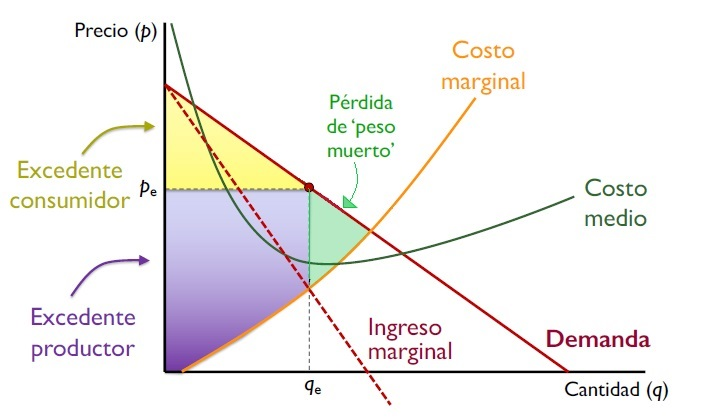
\includegraphics[scale=0.6]{../Figures/Tema_06.42_excedente5.jpg}
\end{frame}

\begin{frame}{Perdida de eficiencia}
    \begin{itemize}
        \item El excedente total en la presencia
        de un monopolista es menor que en el caso de competencia perfecta, y la
        diferencia está dada por el triángulo verde.
        \item La mejora paretiana se
        alcanza si se redistribuye el excedente adicional de tal manera que alguno
        de los agentes esté mejor sin que el otro esté peor.
        \item Bajo monopolio, hay transacciones que no se terminan haciendo y que se hubiesen podido hacer en un contexto de competencia perfecta.
    \end{itemize}
    \begin{boxA}
        El monopolio genera una pérdida de eficiencia puesto que transacciones deseables, que se llevarían a cabo en un contexto de competencia perfecta 
        (ya que el costo marginal es menor a la valoración del consumidor), no son realizadas.
    \end{boxA}
\end{frame}

\begin{frame}{Elasticidad y maximización}
    \begin{itemize}
        \item Los beneficios del monopolio dependen de la elasticidad de la demanda a la que se enfrentan.
        \item ¿Qué sucede en el caso donde la demanda es perfectamente elástica?
        \item Cuanto más inelástica sea la demanda, mas puede aprovechar el monopolista su poder de mercado.
        \item Cuanto más elástica sea la demanda, la pérdida de peso muerto es menor.
    \end{itemize}
    \begin{boxA}
        El poder de mercado del monopolio depende de la elasticidad de
        la curva de demanda. Una curva de demanda más elástica reduce
        el mark-up y la pérdida de eficiencia.

    \end{boxA}
\end{frame}

\begin{frame}{La pérdida de eficiencia del
monopolio depende de la elasticidad de
la demanda}
    \centering
    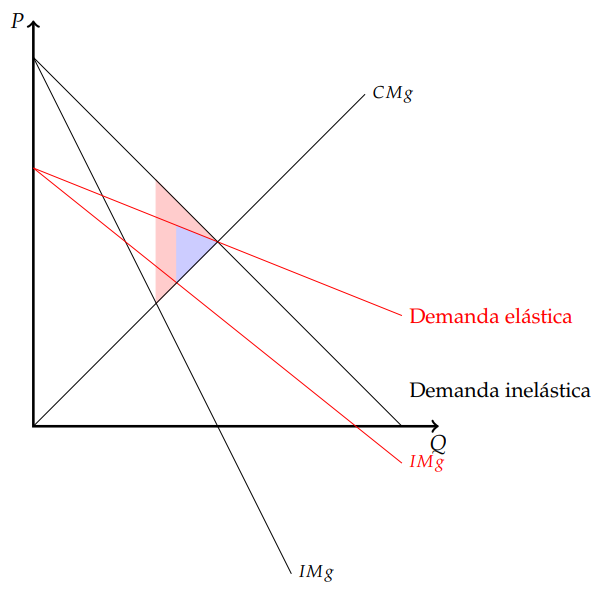
\includegraphics[scale=0.55]{../Figures/C22.9.png}
\end{frame}
\begin{frame}{Poder de mercado}
    \begin{itemize}
        \item El margen de beneficio del monopolista depende de la elasticidad de la demanda.
        \item Esta, a su vez se ve afectada por la competencia.
        \begin{itemize}
            \item Demanda relativamente inelástica si hay pocos sustitutos.
            \item Demanda de bienes esenciales o de primera necesidad también son más inelásticas.
            \item Las empresas con poder de mercado tienen suficiente poder de negociación para fijar los precios sin perder clientes a los competidores.
        \end{itemize}
        \item La política de competencia (antitrust), que limita el poder de mercado, puede beneficiar a los consumidores.
        \begin{itemize}
            \item Por ejemplo, cuando empresas se pueden agrupar en un cartel (poniéndose de acuerdo para mantener precios altos).
            \item La reducción de costos de entrada también puede ser beneficiosa para los consumidores.
        \end{itemize}
    \end{itemize}
\end{frame}

\begin{frame}{Monopolios naturales}
    \begin{itemize}
        \item Hay casos en los cuales el poder monopólico surge de características tecnológicas, de estructura de costos.
        \item El costo marginal es constante y muy bajo.
        \item El costo medio es decreciente. 
        \begin{itemize}
            \item Economías de escala, altos costos fijos, o precios de factores que caen cuanto mas compra la empresa.
            \item Los altos costos fijos imponen barreras a la entrada.
        \end{itemize}
        \item La empresa debe elegir un precio al menos igual al costo medio, que es más alto que el costo marginal.
        \begin{itemize}
            \item ¿Por qué?
        \end{itemize}
        \item En estos casos tenemos un monopolio natural.
        \begin{itemize}
            \item En lugar de fomentar la competencia, el gobierno suele poner controles de precios o hacer estas empresas de propiedad pública.
        \end{itemize}
    \end{itemize}
\end{frame}

\begin{frame}{Monopolio Natural}
    \centering
    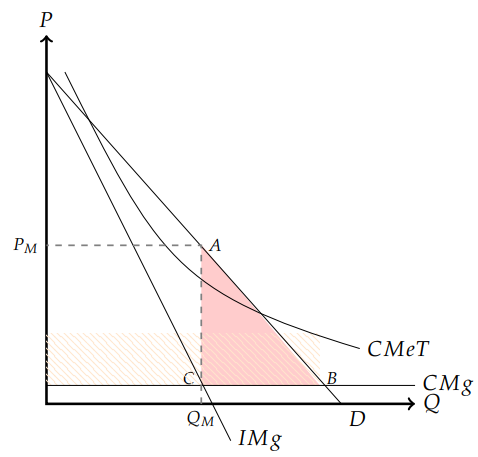
\includegraphics[scale=0.75]{../Figures/C22.10.png}
\end{frame}

\begin{frame}
\frametitle{Casos ideales}
\small
\begin{center}
    \begin{tabular}{c|c}
    \hline
    \hline
    Tomadores de precios & Fijadores de precio \\
    Competencia Perfecta & Monopolio
    \\
    \hline
    \hline
    Puede ser   & Pareto ineficiente \\ 
    Pareto eficiente & (pérdidas peso muerto)
    \\
    \hline
    No hay rentas & Rentas económicas \\
    económicas en & tanto a largo \\
    el largo plazo & como a corto plazo
    \\
    \hline
    Poca gasto en su & Firmas publicitan \\ publicidad & producto único 
    \\
    \hline
    Pocos incentivos para & Firmas invierten en IyD \\ 
    la innovación porque & (tratan de evitar ser \\
    porque otras van a copiar & copiadas)
\end{tabular}
\end{center}
\end{frame}

\begin{frame}
\frametitle{Competencia imperfecta}
\begin{itemize}
    \item La empresa típica se ubica en algún punto entre los casos extremos de la competencia perfecta y el monopolio.
    \item Mercados de competencia imperfecta.
    \begin{itemize}
        \item Oligopolio: sólo hay pocos vendedores, cada uno de los cuales ofrece un producto idéntico o similar a los productos ofrecidos por otros vendedores.
        \item Competencia monopolística: existen numerosas empresas que venden productos similares, pero no idénticos porque logran diferenciarse.
    \end{itemize}
    \end{itemize}
\end{frame}

\begin{frame}
\frametitle{Determinantes de la concentración}
    \begin{itemize}
        \item Costos.
            \begin{itemize}
            \item La existencia de economías de escala hace que solo sobrevivan en el mercado pocas empresas produciendo una gran parte de lo que demanda el mercado. 
            \end{itemize}
        \item Barreras a la entrada .
            \begin{itemize}
            \item Cuando hay barreras a la entrada se bloquea el acceso para que otros empresas ingresen al mercado.
            \end{itemize}
        \item Interdependencia estratégica.
            \begin{itemize}
            \item Cuando las decisiones de una empresa dependen de las decisiones que toman otras empresas. 
            \end{itemize}
    \end{itemize}
\end{frame}

\begin{frame}
\frametitle{Oligopolio}
\begin{itemize}
    \item Competencia entre unas pocas empresas.
    \item Obliga a las empresas a tener en cuenta las reacciones de las competidoras a las desviaciones de los precios de los niveles de producción.
    \item Se introducen consideraciones estratégicas en sus mercados.
\end{itemize}
\end{frame}

\begin{frame}{Oligopolio}
    \begin{center}
      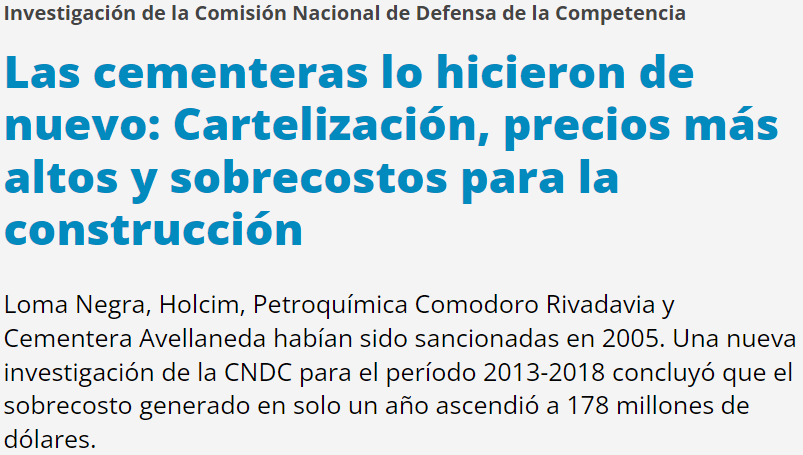
\includegraphics[width=0.75\textwidth]{../Figures/cartel_cementeras.png}
    \end{center}
    \end{frame}

\begin{frame}{Competencia monopolística}
\begin{center}
  \href{https://www.youtube.com/watch?v=po0jY4WvCIc}{
\includegraphics[width=0.75\textwidth]{../Figures/Diferenciacion (1).png}}
\end{center}
\end{frame}

\begin{frame}{Competencia monopolística}
\begin{itemize}
    \item Hay muchos compradores y vendedores\vspace{2mm}
    \item Es fácil entrar y salir\vspace{2mm}
    \item Las empresas toman los precios de las demás como dados\vspace{2mm}
    \item Los productos están diferenciados\vspace{2mm}
    \begin{itemize}
        \item Cada vendedor tiene libertad para subir o bajar los precios debido a la diferenciación de productos.\vspace{1mm}
        \item Entonces, la curva de demanda de cada vendedor tenga pendiente negativa.
    \end{itemize}
    \end{itemize}
\end{frame}

\end{document}
